\appendix
\chapter{Acquisition sequence}
\todo{I'm not sure if this chapter belongs in the appendix. It is kind of a technical thing and I'm not sure where I could fit it in}
\label{ch:acqseq}
During absorption image, the Andor camera will take eight images, which consist of two absorption, two division and four background images (or if the user specifies to only image one species, that then is one absorption and division image and six background images).
% we are not using the macro as I do not need captions or labels and stuff and the image has to be exactly here

As the camera is only interested in the rising edge of the signal, the trigger length is not really important. But the chip will be exposed for the duration of the exposure time, after which the laser should be turned off. The, in our case, 204 pixels are then shifted downwards, taking $t_{vshift}$, which can be calculated by multiplying the vertical shift speed with the pixel height. For the fastest shift speed, this would result in
\begin{equation}
t_{vshift} = \SI{2}{\micro\second\per\px} * \SI{204}{\px} = \SI{408}{\micro\second},
\end{equation}
for the slowest speed we find
\begin{equation}
t_{vshift} = \SI{64}{\micro\second\per\px} * \SI{204}{\px} = \SI{13.1}{\milli\second}
\end{equation}

\draft{acqseq}{Trigger signals}{The triggers are sent as a rectangular signal. The camera will interpret the rising edge of the signal as the starting point of the exposure. Here, $t_{vshift}$ is the time it takes to shift the illuminated pixels downwards, $t_{readout}$ is the time it takes the chip to read out the data and $t_{exposure}$ the exposure time.}

Therefore the four subsequent signals can be taken after
\begin{equation}
t_{trig} = t_{vshift} + t_{exposure}.
\end{equation}
Four images are acquired until the readout process is started. This takes significantly longer, but as explained in \refCh{fast_kin} can be calculated via:
\begin{equation}
t_{ij} = i*vspeed + (i-1)*j_{max}*hspeed+j*hspeed.
\end{equation}
For the whole chip, this gives us $i=4*204=816$, $j=1024$, $j_{max}=1024$, therefore
\begin{equation}
t_{readout} = 816*vspeed + 816*1024*hspeed.
\end{equation}
The trigger signals can finally be calculated via \refTab{trigg_timing}.
\begin{table}
\begin{center}
\begin{tabular}{|l|l|}
	\hline
	\text{\textbf{Trigger number}} & \text{\textbf{Trigger time}} \\ 
	\hline
	\hline
	1 & 0 \\ 
	2 & $t_{trig}$ \\ 
	3 & $2*t_{trig}$ \\ 
	4 & $3*t_{trig}$ \\ 
	5 & $4*t_{trig} + t_{readout}$ \\ 
	6 & $5*t_{trig} + t_{readout}$ \\ 
	7 & $6*t_{trig} + t_{readout}$ \\ 
	8 & $7*t_{trig} + t_{readout}$ \\
	\hline
\end{tabular}
\setCaption{Trigger timing}{The trigger signals are limited by the readout speeds of the chip. This table lists the minimal timings necessary to fully read out the chip. Between signal 4 and 5, the illumated pixels are still shifted downwards, before the chip is read out. This prevents introducing unnecessary errors, as all relevant pixels are then behind the cover of the slit.}
\label{tab:trigg_timing}
\end{center}
\end{table}

\chapter{Shutter circuit}
\label{ch:shutter_circuit}
The circuit given on the next page is the complete circuit as opposed to \refFig{shutter_circuit_simplified}. The key difference here, is that the actual board contains two input/output ports and there are also converters (visible in the top-left corner), that keep the voltage at \SI{24}{\volt}, which is necessary in order to use the MOSFET driver.

The breadboard on the bottom are built into the circuit, so that custom additions can be made, although this is not used in our case.

\begin{figure}[htb]
	\begin{center}
		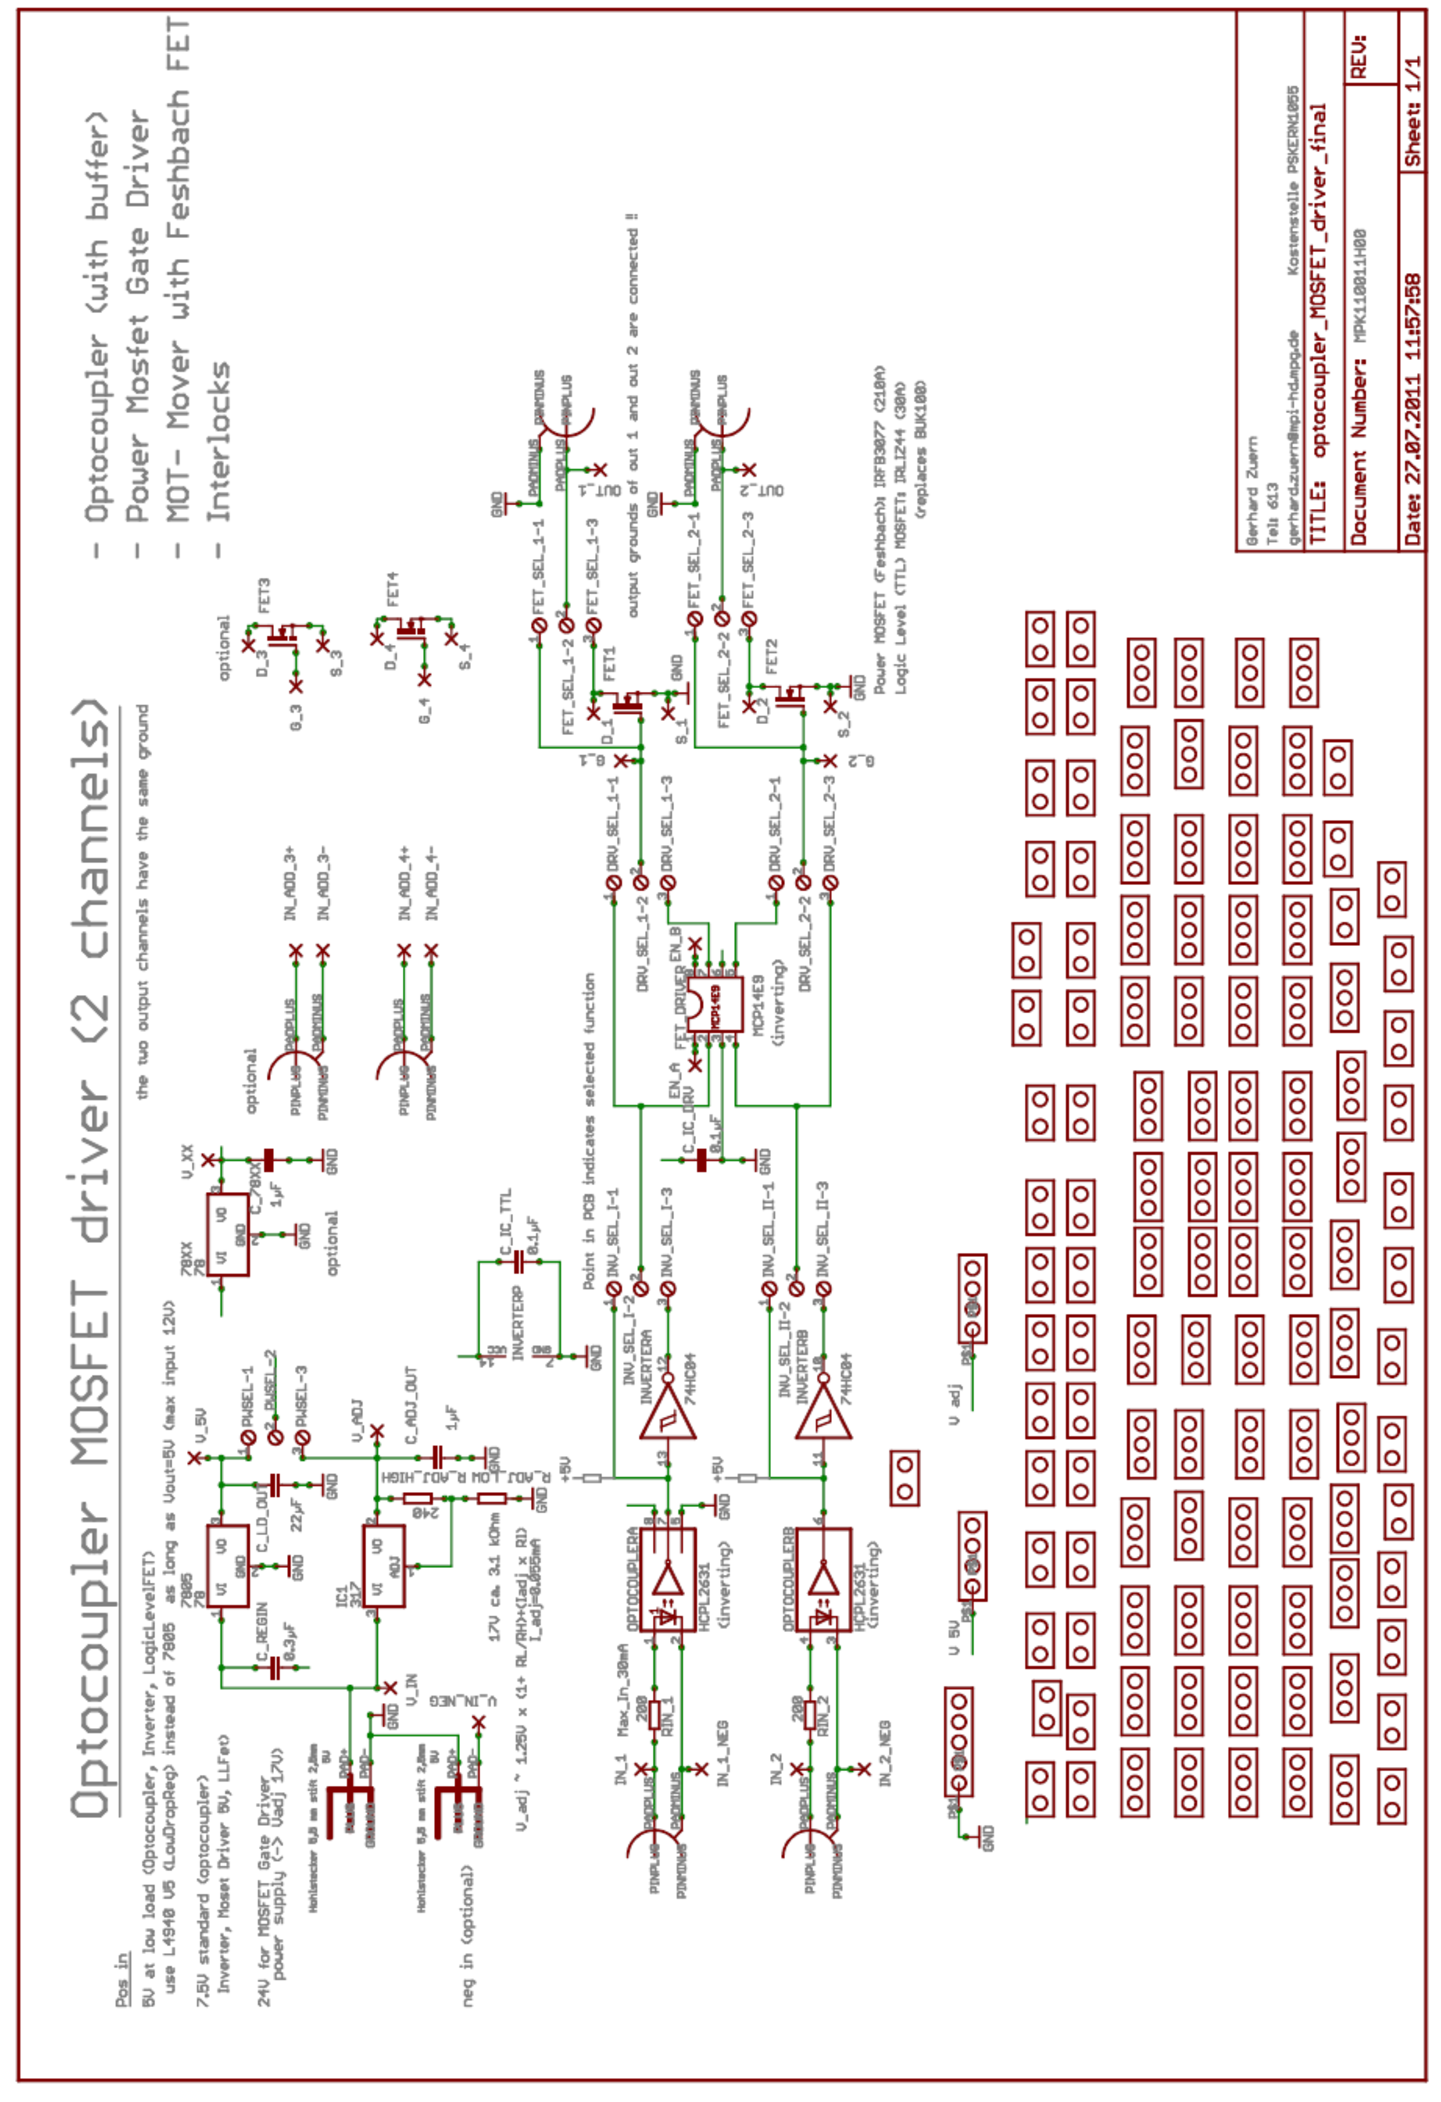
\includegraphics[width=\textwidth]{drafts/shutter_circuit.pdf}
	\end{center}
\end{figure}

\chapter{Setup of the custom slit}

\draft{camera}{Drawing of the camera}{As can be seen in this drawing, the CCD chip is first hidden behind a cover, that also includes an internal shutter and then offset by an additional \SI{5}{\milli\meter}.}

The cover, which can be seen in \refFig{cam_drawing} has a width of \SI{12.5}{\milli\meter}, which adds additional space before the chip. The cover is mainly for a manual cap to cover the chip, when the camera is not used, and an internal shutter. Since we knew, that the internal shutter was not needed, we were able to remove the cover bringing us closer to the chip. Images of under the cover can be found in Appendix \todo{A/B/C? Image?}.

The holes for M4 screws were already there, so a custom plate was built on which the slit could be mounted on.
In the technical drawing in \refFig{cam_drawing}, the centre-most holes are reserved for the slit, which can be moved up and down to select the appropriate height needed for the imaging.
The plate also gives the opportunity to move the whole set with the long holes in the outer-most edges.

It is also important to note, that the camera is very sensitive to stray light. The necessity to cover the laser path is unavoidable, but fortunately a simple solution. The plate offers another set of screw holes, which will hold a SM2-mount, therefore eliminating any gap that could allow photons to reach the camera externally.

The long path of SM2 tubes then only allows the smallest amount of stray light to enter the camera, which will have significantly lower intensity than the actual absorption image.